%%%%%%%%%%%%%%%%%%%%%%%%%%%%%%%%%%%%%%%%%%%%%%%%%%%%%%%%%%%%%%%%%%%%%%%%%%%%
%% Author template for Interfaces (inte)
%% Mirko Janc, Ph.D., INFORMS, mirko.janc@informs.org
%% ver. 0.95, December 2010
%%%%%%%%%%%%%%%%%%%%%%%%%%%%%%%%%%%%%%%%%%%%%%%%%%%%%%%%%%%%%%%%%%%%%%%%%%%%
%\documentclass[inte,blindrev]{informs3}
\documentclass[inte,nonblindrev]{informs3} % current default for manuscript submission

%\OneAndAHalfSpacedXI
\OneAndAHalfSpacedXII % Current default line spacing
%%\DoubleSpacedXII
%%\DoubleSpacedXI

% If hyperref is used, dvi-to-ps driver of choice must be declared as
%   an additional option to the \documentclass. For example
%\documentclass[dvips,inte]{informs3}      % if dvips is used
%\documentclass[dvipsone,inte]{informs3}   % if dvipsone is used, etc.

% Private macros here (check that there is no clash with the style)

% Natbib setup for author-year style
\usepackage{natbib}
 \bibpunct[, ]{(}{)}{,}{a}{}{,}%
 \def\bibfont{\small}%
 \def\bibsep{\smallskipamount}%
 \def\bibhang{24pt}%
 \def\newblock{\ }%
 \def\BIBand{and}%
 
\usepackage{flexisym}
\usepackage[utf8]{inputenc}
\usepackage[english]{babel}
\usepackage{multirow}
\usepackage{amssymb}% http://ctan.org/pkg/amssymb
\usepackage{pifont}% http://ctan.org/pkg/pifont

%% Setup of theorem styles. Outcomment only one. 
%% Preferred default is the first option.
\TheoremsNumberedThrough     % Preferred (Theorem 1, Lemma 1, Theorem 2)
%\TheoremsNumberedByChapter  % (Theorem 1.1, Lema 1.1, Theorem 1.2)

%% Setup of the equation numbering system. Outcomment only one.
%% Preferred default is the first option.
\EquationsNumberedThrough    % Default: (1), (2), ...
%\EquationsNumberedBySection % (1.1), (1.2), ...

% In the reviewing and copyediting stage enter the manuscript number.
\MANUSCRIPTNO{040-05-19-OM} 
% When the article is logged in and DOI assigned to it,
%   this manuscript number is no longer necessary

\setcounter{secnumdepth}{0}% "Interfaces" does not number sections

%%%%%%%%%%%%%%%%
\begin{document}
%%%%%%%%%%%%%%%%

% Outcomment only when entries are known. Otherwise leave as is and 
%   default values will be used.
%\setcounter{page}{1}
%\VOLUME{00}%
%\NO{0}%
%\MONTH{Xxxxx}% (month or a similar seasonal id)
%\YEAR{0000}% e.g., 2005
%\FIRSTPAGE{000}%
%\LASTPAGE{000}%
%\SHORTYEAR{00}% shortened year (two-digit)
%\ISSUE{0000} %
%\LONGFIRSTPAGE{0001} %
%\DOI{10.1287/xxxx.0000.0000}%

% Author's names for the running heads
% Sample depending on the number of authors;
% \RUNAUTHOR{Jones}
% \RUNAUTHOR{Jones and Wilson}
% \RUNAUTHOR{Jones, Miller, and Wilson}
\RUNAUTHOR{Abdollahnejadbarough et al.} % for four or more authors
% Enter authors following the given pattern:
%\RUNAUTHOR{}

% Title or shortened title suitable for running heads. Sample:
\RUNTITLE{Verizon Uses Advanced Analytics to Rationalize its Tail Spend Suppliers}
% Enter the (shortened) title:
%\RUNTITLE{040-05-19-OM}

% Full title. Sample:
\TITLE{Verizon Uses Advanced Analytics to Rationalize its Tail Spend Suppliers}
% Enter the full title:
%\TITLE{}

% Block of authors and their affiliations starts here:
% NOTE: Authors with same affiliation, if the order of authors allows, 
%   should be entered in ONE field, separated by a comma. 
%   \EMAIL field can be repeated if more than one author
\ARTICLEAUTHORS{
\AUTHOR{Hossein Abdollahnejadbarough, Kalyan S. Mupparaju, Sagar Shah, Colin P. Golding,  Abelardo C. Leites, Timothy D. Popp, Eric Shroyer, Yanai S. Golany, Anne G. Robinson, Vedat Akgun}
\AFF{Verizon, One Verizon Way, Basking Ridge, NJ 07920, United States \\ \EMAIL{{hossein.abdollahnejadbarough@verizon.com, kalyan.sashank.mupparaju@verizonwireless.com, sagar.shah2@verizonwireless.com, colin.golding@ie.verizon.com, abelardo.c.leites@one.verizon.com, timothy.popp@verizon.com, eric.shroyer@verizon.com, yanai.golany@verizonwireless.com, anne.robinson@verizonwireless.com, vedat.akgun@verizonwireless.com}}
}
}

\ABSTRACT{Verizon Global Supply Chain organization currently manages thousands of active supplier contracts. These contracts account for several billion dollars of annualized Verizon spend. Managing thousands of suppliers, controlling spend and achieving the best price per unit (PPU) through negotiations are costly and labor intensive tasks handled by Verizon strategic sourcing teams. Verizon engages thousands of suppliers for many reasons – best price, diversity, short term requirements, etc. While managing a few larger spend suppliers can be done manually by dedicated sourcing managers, managing thousands of smaller suppliers at the tail spend is challenging, can often introduce risk, and can be expensive. At Verizon, a unique blend of descriptive, predictive and prescriptive analytics as well as Verizon-specific sourcing acumen was leveraged to tackle this problem and rationalize Verizon’s tail spend suppliers. Through the creative application of Operations Research, Machine Learning, Text Mining, Natural Language Processing and Artificial Intelligence, Verizon reduced spend by millions of dollars and acquired lowest PPU for the sourced products and services. Other benefits Verizon realized were centralized and transparent contract and supplier relationship management, overhead cost reduction, decreased contract execution lead time, and service quality improvement for Verizon’s strategic sourcing teams.
}

% Fill in data. If unknown, or unnecessary, outcomment the field
\KEYWORDS{Global Procurement, Strategic Sourcing, Supplier Rationalization, Business Process Outsourcing, Spend Analytics}
\HISTORY{}

\maketitle
%%%%%%%%%%%%%%%%%%%%%%%%%%%%%%%%%%%%%%%%%%%%%%%%%%%%%%%%%%%%%%%%%%%%%%

% Samples of sectioning (and labeling) in INTE
% NOTE: (1) \section and \subsection do NOT end with a period
%       (2) \subsubsection and lower need end punctuation
%       (3) capitalization is as shown (title style).
%
%\section{Introduction.}\label{intro} %%1.
%\subsection{Duality and the Classical EOQ Problem.}\label{class-EOQ} %% 1.1.
%\subsection{Outline.}\label{outline1} %% 1.2.
%\subsubsection{Cyclic Schedules for the General Deterministic SMDP.}
%  \label{cyclic-schedules} %% 1.2.1
%\section{Problem Description.}\label{problemdescription} %% 2.

% Text of your paper here
\section{Introduction}
Verizon is a multi-billion dollar telecommunication and media company with global operations and diverse product offerings such as Huffington Post, FiOS, AOL, Yahoo! and Visible, more than 150,000 employees worldwide and 2,300 retail stores in the United States. Verizon is a pioneer in commercializing 5G internet services and operates the world's largest cellphone network, covering personal, residential and business customers. To be able to run the world's fastest telecommunications network and provide a world-class customer experience to its customers, Verizon utilizes the latest and most advanced technologies available in the market. As a result, partnering with global telecommunication equipment manufacturers has been a successful business strategy for Verizon to deliver its services across the globe.

Since delivering quality services at the lowest possible price to customers is Verizon's corporate strategy, Verizon implemented world-class intelligent systems within its global strategic sourcing teams, leading to significant cost reductions in acquired network equipment and services, managing redundancies and improving its Cost-To-Serve (CTS) model.

Operating a network with millions of subscribers calls for strong risk avoidance strategies. A small disruption in supply of network equipment or maintenance components might lead to a drop in network services and significant customer losses. Therefore, Verizon avoids single sourcing its telecommunication equipment and services from its suppliers and instead, engages multiple suppliers per category for its required products and services. Supplier diversification programs, which were implemented by Verizon's strategic sourcing teams in early 2000s, allow competitive pricing, risk and supply disruption management. While these programs were successful at the beginning, they increased Verizon's supplier network to approximately 47,000 suppliers worldwide over time, leading to significant contract management, supplier negotiations and overhead costs for the sourcing teams to the point that these costs were exceeding the programs' benefits. As a result, in late 2017 Verizon decided to transform its sourcing operating model and initiated one of the largest public business transformation efforts in the history of the telecommunications industry.

Deciding on the right number of large and small suppliers is a challenging business decision for any organization with global sourcing operations. Conducting multiple Request for Proposals (RFPs) and several rounds of supplier negotiations often takes thousands of supplier business attributes into consideration, creating opportunities to leverage advanced analytics techniques and transforming traditional decision making processes into a more intelligent and data-oriented approaches. 

In order to define the business problem which is addressed in this paper effectively, first, the dynamics of global strategic sourcing and procurement operations is explained. In addition, a brief description of the electronics manufacturing and the telecommunications business is also provided.

\subsection{Strategic Sourcing and Global Procurement}
Successful global organizations focus their effort and talent on their core business and use outsourcing for non-core business activities. At Verizon, the focus is on the network and technology. For instance, 4G and 5G networks, fiber optic broadband services and media content creation and delivery. Any business operations which is not within Verizon's core business expertise will be outsourced to qualified vendors and suppliers. This practice is known as \textit{indirect procurement}. On the other hand, in order to run the network and communication towers, Verizon uses a variety of fiber optic cables, electronic boards, switches and routers which are sourced from well-known electronic manufacturers and suppliers. This approach is known as \textit{direct procurement} and suppliers in this category are often treated as strategic business partners with business models such as gain sharing and transparent pricing. In general, sourcing products and services which are used within the products and services a company sells directly is direct procurement and everything else is indirect procurement. 

At Verizon, Global Strategic Sourcing teams and category sourcing managers are responsible for supplier selection, evaluation, negotiations and contracting for the above-mentioned procurement strategies. Negotiating contracts is time consuming, as it involves a strong detailed financial analysis, planning and coordination, legal, compliance and global clearance reviews. As a result, contract negotiation lead times can vary from a few days to a few years depending on complexity of the contract terms and monetary value of the contract. In addition, sourcing operations often impact company's Profit and Loss (P\&L) statement and financial earnings which require Financial Planning and Analysis (FP\&A). 

In order to evaluate strategic sourcing operations, Key Performance Indicators (KPIs) are defined by Verizon's FP\&A teams. These indicators are often used to benchmark sourcing organization's effectiveness in comparison to other internal and external organizations industry wide. Table \ref{tabel:tbl1} lists and defines the important KPIs which are used by the Verizon strategic sourcing and FP\&A organizations for reporting and financial analysis. At Verizon, a sourcing operation starts with a Sourcing Request Form (SRF), submitted by a business unit. A supplier Master Agreement (MA), an Agreement (AGR) or a contract Amendment is the output of successful sourcing operations. A Category Sourcing Expert (CSE), manages multiple SRFs at a time for one or multiple sourcing categories. CSEs often conduct a Request for Information (RFI), a Request for Proposal (RFP), a Request for Quote (RFQ) or a Request for Bid (RFB) to identify proper suppliers. Conducting an RFX, where X could be either one of the previously mentioned requests, could take anything between a few weeks to a few months to complete. Depending on the RFX's result, CSEs might decide to sign a contract with an existing supplier or onboard a new supplier to the supplier network.

\begin{table}
	\begin{tabular}
		{c | >{\centering\arraybackslash}m{3.5 cm} | >{\centering\arraybackslash}m{10 cm}}
			\multicolumn{3}{c}{} \\
			\hline
			Metric Type & KPI & Definitions \\ 
			\hline
			\multirow{7}{*}{Operational} 
				& SRF Lead Time & Time between an SRF and contract execution \\
				& SRF Hold Time & Waiting time for an SRF approval by internal business unit executives\\ 		
				& Number of RFX Conducted & Total Number RFXs conducted by CSEs \\		
 				& Number of MAs & Total supplier master agreements negotiated \\
 				& Number of AGRs & Total agreements or amendments negotiated \\
 				\hline
			\multirow{8}{*}{Financial} 
				& ROI per CSE & Sourcing Return On Investment (ROI) per CSE\\
 				& Managed Spend & Company spend managed by sourcing teams \\
 				& PPU & Year-over-year price per unit of sourced categories \\ 
 				& Commodity Maturity & Level of procurement efficiency for a sourced commodity \\
 				& Savings \% & Percentage of spend savings compared to baseline (prior year spend) \\
			\hline
	\end{tabular}
	\caption{Important KPIs for Strategic Sourcing}
	\label{tabel:tbl1}
\end{table}

\subsection{Original Equipment Manufacturer (OEM) and Value Added Reseller (VAR)}
Within electronics manufacturing, manufacturers can also choose to manufacture everything related to their products in-house or source from other manufacturers. The term Original Equipment Manufacturer (OEM) is often referred to as the original manufacturer of an electronic product, part, component or software. Large electronics manufacturers often use smaller manufacturer's microprocessors and other components in their products. To keep track of their Bill Of Material (BOM), these manufacturers either over-write the OEM number, a unique identifier to a product, of these smaller components with their own OEM number or use a Manufacturer Part Number (MPN) instead. Telecommunication companies such as Verizon often use these OEM numbers or MPNs in their procurement while financial systems as unique identifiers of the sourced items for reporting and planning purposes. Verizon network planning teams usually refer to these identifiers to plan for network spend and project management activities and accounting teams use them for taxing and bookkeeping. There are other use cases for this information, for example in contract management, product price variance analysis and negotiations with the suppliers. 

Total spend with a supplier is a good reference point to start contract negotiations. However, deciding on the total spend with a supplier requires visibility to all the OEM numbers within a sourced product and the ability to trace the supplier spend at the OEM level. Enterprise Resource Planning (ERP) systems often fail to address the need for this information as most of them are built for general purposes and not customized to telecommunication business needs. For instance, when Verizon initiates a Purchase Order (PO) to a vendor, the required OEM or MPN information is often sent to the vendor via emails or as an attachment to the PO, generating large unstructured data within ERP data warehouses. The sourcing teams would need to refer to these files or PO attachments through manual search, for any internal financial analysis, project planning and vendor auditing through manual searches.

The sourcing channel may also cause missing or inconsistent OEM information in ERP systems as well. Large companies often choose to engage numerous suppliers to source the same category for various reasons – best price, portfolio diversity, short term requirements and risk management are some of these reasons. Some of these suppliers are resellers of OEM products. Therefore, the same product or service can be sourced from either the OEM or a VAR. VARs often carry inventory holding risks for their customers (e.g. Verizon) but demand large profit margins when negotiating with OEMs and their customers in return. Inventory holding risks are often the cause of product price variances between VARs and OEMs. If an item is procured through a VAR, depending on the VAR's ERP system data governance, the OEM information might not be captured by the VARs. Thus, the VAR might not be able to pass them on to Verizon which could complicate the OEM's total spend calculation.  

The procurement challenges Verizon faces today are industry wide and not unique to the Verizon business model. To name a few, Business Process Outsourcing (BPO) \citep{r26}, wholesaling, automobile manufacturing, pharmaceutical distribution and even start-up \citep{r25} businesses are always exposed to inconsistent data governance, decentralized decision making, lack of visibility on end-to-end pricing decisions and supplier negotiations. Although the business problem addressed in this paper focuses on rationalizing tail spend suppliers, the Verizon Supplier Rationalization Tool (VSRT) developed to solve this problem can be applied to suppliers of any spend size or industry, providing valuable information to their procurement teams and speeding up contract execution.

The structure of this paper is as follows: A survey of existing supplier rationalization works using data analytics is provided in the Literature Review section. The business goals and explanation of the business environment are provided in the Business Goals and Environment section. Topics related to the machine learning algorithms and optimization methods used in VSRT to solve this problem are covered in the Solution Methodology section. A review of the VSRT implementation results are provided in the Solution Results section. Final remarks about this end-to-end VSRT solution are provided in the Conclusion section. 

\section{Literature Review}
Supplier evaluation has been mainly addressed in the literature using conceptual, empirical or quantitative models. \cite{r17} reviewed most of the available conceptual and empirical models briefly covered some of the available quantitative techniques. With the recent advancements in machine learning and big data technologies, decision makers are more interested in \textit{prescriptive} techniques, therefore, conceptual and most of the available empirical models in the literature have become impractical. Table \ref{table:tbl2a} provides a high level comparison of the tools, techniques and algorithms, between the existing literature and the VSRT. In order to have a consistent comparison, four major capabilities are used for comparison: Data processing engine, supplier evaluation engine, supplier ranking algorithm and reporting/visualization engines. 

\newcommand{\xmark}{\ding{55}}
%\checkmark

\begin{center}
	\begin{table}
		\begin{tabular}{>{\centering\arraybackslash}m{4.0 cm} | 
						>{\centering\arraybackslash}m{2.0 cm} | 
						>{\centering\arraybackslash}m{3.0 cm} |
						>{\centering\arraybackslash}m{3.5 cm} |  
						>{\centering\arraybackslash}m{2.5 cm}
						}
			\multicolumn{5}{ c } {}\\
			\hline
			Publication & Data Processing Engine & Supplier Evaluation Engine 
			& Supplier Ranking Algorithm & Reporting \& Visualization Engines\\ 
			\hline
			\multirow{5}{*}{} 
			\cite{r19} & \xmark & DEA without KPIs & \xmark & \xmark \\
			\cite{r20} & \xmark & DEA & \xmark & \xmark \\
			\cite{r17a} & \xmark & DEA & \xmark & \xmark \\
			\cite{r33} & \xmark & DEA & Performance Diversity Index & \xmark \\
			\cite{r28} & \xmark & DEA \& Monte Carlo & Hierarchy Base & \xmark \\
			\cite{r27} & \xmark & Probabilistic Models (Erlang) & \xmark & \xmark \\			
			\cite{r31} & \xmark & MIP (Minimax) & \xmark & \xmark \\			
			\cite{r29} & \xmark & MIP \& Fuzzy Theory & \xmark & \xmark \\			
			\cite{r22} & \xmark & Fuzzy Theory & Weighted Average & \xmark \\			
			\cite{r30} & \xmark & Fuzzy Theory & Fuzzy Preference Index & \xmark \\
			\textbf{Verizon Supplier Rationalization Tool (VSRT)} & \textbf{NLP \& RNN} & \textbf{Clustering \& Inverse DEA with KPIs} & \textbf{TOPSIS \& Shannon Entropy} & \textbf{Interactive Visualization} \\
			\hline
		\end{tabular}
		\caption{Capability Comparison Between VSRT and Existing Literature}
		\label{table:tbl2a}
	\end{table}
\end{center}

The majority of the existing quantitative models in supplier evaluation are utilizing Data Envelopment Analysis (DEA) \citep{r12}. DEA is a well-known optimization technique used for benchmarking manufacturing and service business units with their peer units, known as Decision Making Units (DMUs). \cite{r19} used DEA to monitor the performance of a single supplier over time. \cite{r20} expanded the use of DEA models for supplier evaluation and included operational and strategic KPIs within their model, however, their model was focused only on manufacturing industries, did not cross-evaluate supplier based on different categories and was not useful for evaluating service providing suppliers. The first DEA model which cross-evaluated suppliers was intorduced by \cite{r17a}. Similar to \cite{r20}, this model was only utilizing operational KPIs as well. 

Identifying candidate suppliers for rationalization can be formulated into a Mixed Integer Programme (MIP) \citep{r34}. An MIP has an objective function which could minimize or maximize the impacts of supplier rationalization on the business subject to various business constraints. \cite{r32} formulated an MIP to choose the optimal terms for contracts such as contract duration and product order quantities in the presence of market price uncertainty, supplier discounts, investment costs and supplier capacity constraints.

Recent academic works in supplier evaluation cover areas such as evaluating suppliers at the sourcing category level \citep{r22}, sourcing services \citep{r23} and public procurement \citep{r24}. Supplier risk management concept \citep{r27} was also added to supplier evaluation techniques using probabilistic functions derived from an Erlang or a Normal distribution function. For instance, \cite{r28} included Value-At-Risk calculations and \cite{r29} incorporated an Auction theory mechanism within their models to shortlist suppliers before evaluation. Other quantitative techniques such as Multi-Objective Goal Programming (MOGP) \citep{r31} where suppliers were evaluated based on multiple business objectives or \citep{r30} where the likelihood of suppliers meeting their target KPIs were modeled using fuzzy numbers, have also been introduced in the recent supplier evaluation models.

Processing large volumes of unstructured supplier data has been a major shortcoming of the existing literature. All of the existing supplier evaluation techniques would require significant manual data processing and computation time to provide insights on suppliers. In today's business world where speed and agility to provide insights to decision makers are critical for successful negotiations, spending time and resources on processing supplier data will make the existing models in the literature impractical. VSRT includes a data pre-processing engine which leverages Natural Language Processing (NLP) \citep{r10} and Recursive Neural Networks (RNN) \citep{r5} to build high quality data models. These data models are used within other stages of the solution to reduce computation time, user interaction time with the solution and provide quality results. The data processing capability will also help with scenario analysis, tool reliability and user experience.  

Majority of the existing supplier evaluation techniques are either missing critical factors such as strategic KPIs or provide non-deterministic results which are often difficult to explain to business users, are not objective, do not assign different weights to influential sourcing parameters, lack comparison with alternative suppliers and do not address supplier performance at the sourcing category level. Deploying a solution with these shortcomings is risky for any businesses regardless of their size or industry. In addition, none of the existing literature focus on the tail spend suppliers. Unlike the existing literature, the VSRT clusters suppliers based on their business attributes and cross-evaluates them within their own cluster. This allows the VSRT's supplier evaluation engine to perform complex computations on a large volume of supplier data, scaling up the solution on the entire supplier base and provide deterministic results which are simple to explain to the business users.

Similar to VSRT, \cite{r33} provided a DEA model to evaluate suppliers with their peers, however, following their DEA model, they used a supplier Performance Diversity Index (PDI) to rank the rationalization candidates. This new approach was tested on published datasets. The results were compared to an existing ranking method, Maverick Index \citep{r21}, which uses the mean of suppliers' efficiency score to rank suppliers. They concluded that evaluating suppliers using both MIP and PDI in tandem helps identifying suppliers which not only excel with respect to their peers but also offer a unique set of capabilities which other suppliers lack. \cite{r30} also used a Fuzzy Preference Index (FPI) \citep{r36} to rank suppliers based on a set of fuzzy numbers. The VSRT ensures that suppliers which provide similar sourcing categories are compared with their peers by clusters them according to their business attributes, then applies a supplier ranking algorithm to identify the rationalization candidates. The Technique for Order Preference by Similarity to Ideal Solution (TOPSIS) \citep{r4}, which is a data-driven ranking algorithm, is combined with the Shannon Entropy \citep{r6} to rank suppliers and identify the rationalization candidates subject to multiple business criteria. The VSRT approach is superior to the existing literature as it is unbiased, data oriented and can be customized according to the CSE needs. 

The interactive reporting and visualization provided by the VSRT have not been within the scope of any of the existing literature. However, for a successful solution deployment, interactive reports and visualization are key to communicate complex information and recommendations. VSRT equips sourcing teams with several detailed reports at both category and SKU levels, providing spend visibility for all the OEMs within the supplier network. 

\section{Business Goals, Environment and Assumptions}
\subsection{Tail Spend Definition}
Figure \ref{fig:fig1} is a Pareto chart showing Verizon aggregated supplier spend where larger spend suppliers, known as Head Spend suppliers, appear to the left on the chart, while others known as Tail Spend suppliers, appear to the right. The definition of tail spend can be quite abstract since in practice, the head of the tail spend (Suppliers 28, 19, 14 and 11) is hard to differentiate from the head spend suppliers. For large organizations like Verizon, a supplier with annual spend of \$5 million might be considered tail spend supplier, whereas for smaller companies, the cap might be a lot lower. The long tail suppliers (Suppliers 27 and so on) are a lot harder to rationalize and consolidate than the head of the tail suppliers, as these suppliers could be niche, offering products or services which are important for Verizon's business or have geographical representation and strategic advantages. 

\begin{figure}
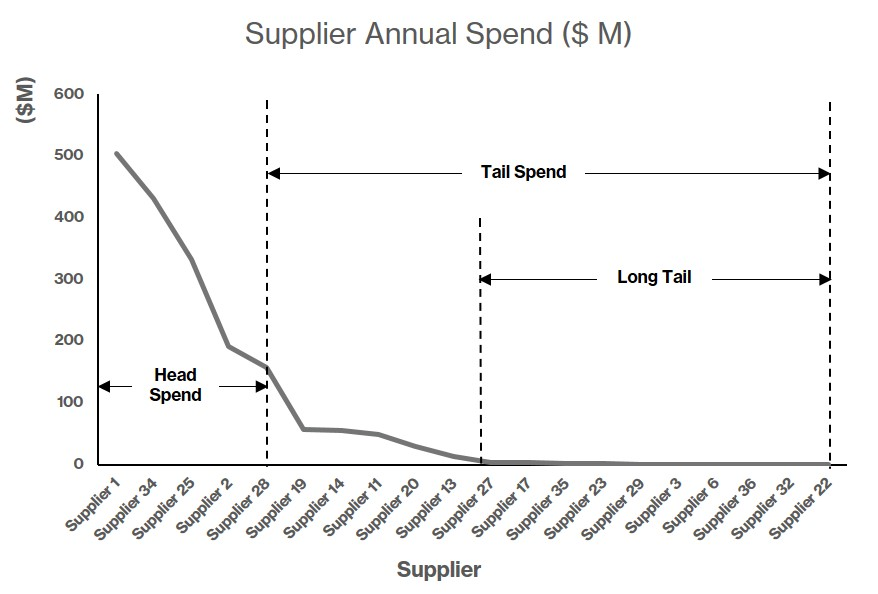
\includegraphics[width = 0.8\textwidth]{TailSpendBW.jpg}
\caption{Tail Spend Suppliers}
\label{fig:fig1}
\end{figure}

\subsection{Business Environment}
Consider a business environment where there are multiple suppliers (or OEMs) per sourcing category and different sourcing channels, e.g. a business can source their products and services either directly from the OEMs or from VARs. In addition, a supplier can use other OEMs' products or services to create a new product, build kits or provide service and product bundles to a business. Figure \ref{fig:fig1a} illustrates this business environment. The decision on which sourcing channel or supplier to choose and source from is a function of several factors: PPU of the products and services, discounts, bundled/tiered pricing, order volume consolidation, delivery date and location of ordered items, previous agreements with the vendors or OEMs, and even tariffs and corporate taxes are among these factors. For simplicity, these factors can be assigned to two major classifications: Pricing and Quality Metrics (KPIs).

\subsection{Business Goals}
The primary goal of the VSRT is to provide insights to the sourcing teams to rationalize Verizon's tail spend suppliers. More specifically this solution aims to provide data-driven tools and capabilities to:

\begin{enumerate}
\item Reduce the number of tail spend suppliers and supplier management overhead costs
\item Identify a subset of suppliers which provide products and services that minimize the overall Verizon spend while maximize the quality metrics 
\item Recommend alternative suppliers, from the head spend supplier set, to take over the tail spend supplier's order volume and consolidate order quantities
\end{enumerate}

\begin{figure}
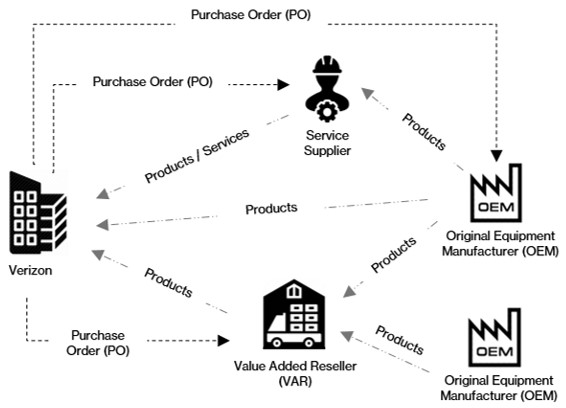
\includegraphics[width = 0.8\textwidth]{BusinessEnv.jpg}
\caption{Verizon Sourcing Business Environment}
\label{fig:fig1a}
\end{figure}

\subsection{Assumptions and Definitions}
Achieving the above mentioned goals requires some business assumptions:
\begin{itemize}
\item At least two active suppliers per category are already in the Verizon supplier network
\item No new supplier is added to the network for any of the categories under study
\item Suppliers are able to add categories which they are not currently covering in their offerings, which is subject to supplier negotiations
\end{itemize}

This decision making problem can be translated into mathematics. Definition 1 in Appendix A defines this problem as: There should be a subset of suppliers, $s\textprime$, where their KPIs and PPUs are competitive with others in almost all sourcing categories. To avoid this supplier subset being empty, Verizon always prioritizes quality over pricing. To create this subset of suppliers and achieve the above-mentioned goals, transaction level spend data as well as other data sources need to be analyzed. Since the data size for transaction level data can be quite large, traditional data analysis techniques will not be able to solve this decision making problem fast enough and provide business insights for decision makers. Therefore, different types of analytics and algorithms were combined in an innovative sequence to tackle this problem. Next section will cover details of this unique approach.

\section{Solution Methodology} 
The Verizon Supplier Rationalization Tool (VSRT) methodology consists of four main stages: Data Models, Machine Learning Models, Optimization Models and Interactive Visualizations. Figure \ref{fig:fig2} shows these stages where different models were applied and the departments impacted by each within VSRT. The solution's analytics journey starts with structuring transaction level invoice line and PO data, blending them with external structured datasets and build data models. Using the data models, the Machine Learning engine clusters suppliers based on their business attributes. The Optimization Engine uses an inverse DEA model to evaluate suppliers within each cluster with their peers and creates a supplier efficiency score matrix. A TOPSIS algorithm which uses Shannon Entropy and the suppliers' efficiency score matrix, ranks the suppliers and identifies the rationalization candidates. Results are reported to the decision makers using Interactive Visualization. The outputs of each stage are inputs of the  next stage. Figure \ref{fig:fig2Journey} explains the details of these stages as well as the functionality of each stage. Since data models are critical components of any analytical solution, first, the data models are explained.

 
\begin{figure}
	%\centering
	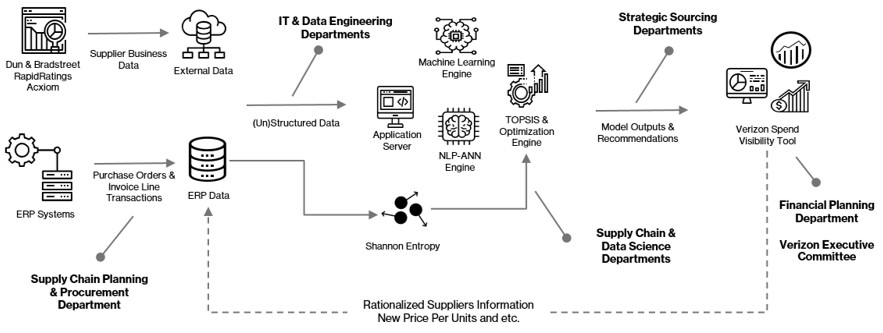
\includegraphics[width=1.0\textwidth]{FlowGraph.jpg}
    \caption{The VSRT Models, Data Flow and Covered Business Departments}
    \label{fig:fig2}
\end{figure}


\begin{figure}
	%\centering
	%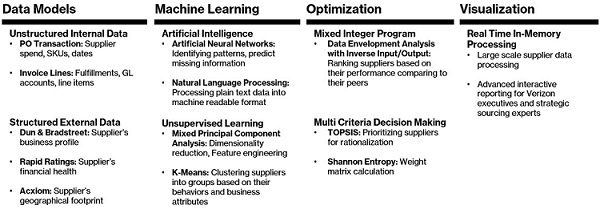
\includegraphics[width=1.0\textwidth]{Journey.jpg}
	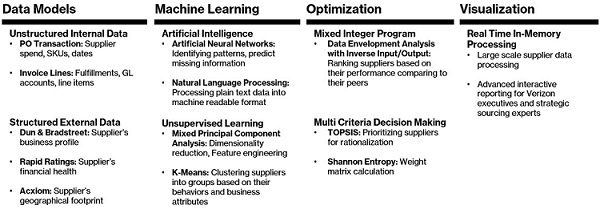
\includegraphics{Journey.jpg}
    \caption{The VSRT Analytics Journey}
    \label{fig:fig2Journey}
\end{figure}

\subsection{Data Models}
A blend of Verizon internal and external (third party) data sources was used to build supplier business profiles. For the internal data sources, transaction level PO and invoice line data generated by Verizon's ERP systems were used. ERP data warehouses were often filled with enormous quantities of unstructured data, where key data elements such as OEM numbers/names, MPN, spend classifications and taxonomies are either missing or mislabeled. That being said, NLP was used to tokenize transaction level PO and invoice line data to extract key information and fill in missing data. 

A set of RNNs was built followed by the NLP text mining results to predict spend categories or relabel the existing data, OEM names or MPNs if needed. The developed RNN models have multiple hidden layers and were trained and retrained iteratively on high quality datasets provided by OEMs until their accuracy reached 98\% (i.e. 98\% of the time the RNN was able to predict the exact missing information as the OEM provided information). Figure \ref{fig:fig2RNN} illustrates the sequence of NLP and RNN models and details about their configurations used to predict or relabel missing information within the Verizon ERP datasets.

\begin{figure}
	%\centering
	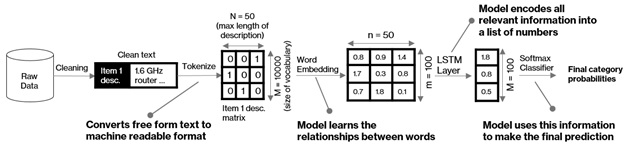
\includegraphics[angle=0, width=1.0\textwidth]{RNN.jpg}
    \caption{Natural Language Processing and Recurring Neural Network Used to Predict Missing Data}
    \label{fig:fig2RNN}
\end{figure}

External data sources also were added to the structured supplier spend data to build the suppliers' Business Attribute Matrix (BAM). Financial and market intelligence datasets from external sources including Dun \& Bradstreet, RapidRatings and Acxiom along with other datasets such as suppliers' geo-footprint, diversity, compliance, risk and capabilities were added to enrich the structured spend data and strengthen the overall analysis. Table \ref{table:tbl2} shows important examples of the data sources and type of variables used to build the supplier BAM. The complete list of these variables is exhaustive and proprietary to Verizon. Hadoop Super Cluster and Hive platforms were used as a System of Records (SOR) to host and process all data models. The outputs of this stage are structured high quality supplier business data which can be consumed by Machine Learning models in the next stage. In addition,  high level business reporting and spend analysis can be built with the outputs of this stage. 

\begin{center}
	\begin{table}
		\begin{tabular}{>{\centering\arraybackslash}m{2.0 cm} | 
						>{\centering\arraybackslash}m{2.5 cm} | 
						>{\centering\arraybackslash}m{7 cm} | 
						>{\centering\arraybackslash}m{4 cm}
						}
			\multicolumn{4}{ c } {}\\
			\hline
			Source & Category & Example(s) & Data Type \\ 
			\hline
			\multirow{5}{*}{Internal} 
				& Spend & YoY Spend, Sourcing Category & Integer, Categorical \\
 				& Items & OEM Number, MPN, Item Description & Categorical \\
 				& Diversity & Portfolio or Workforce Diversity & Binary \\
 				& Accounting & Sourceable or Non-Sourceable Spend & Binary, Integer \\ 
			\hline
			\multirow{4}{*}{External} 
				& Acxiom & Geographic, Socioeconomic, Demographic & Integer, Categorical, Binary \\
 				& RapidRatings & Financial Health, Risk & Integer, Categorical \\
 				& Dun \& Bradstreet & Financial Ratings, Market Intelligence & Integer, Categorical \\ 
			\hline
		\end{tabular}
		\caption{Main Data Sources Used in VSRT}
		\label{table:tbl2}
	\end{table}
\end{center}

\subsection{Machine Learning Models}
Assume there are $S$ tail spend suppliers with $M$ business attributes per supplier where Verizon sources $C$ distinct sourcing categories. The suppliers' BAM will have $S$ rows and $C \times M$ columns. If creating a combination of these attributes, i.e. ${C \times M}\choose{k}$ where $k$ is the number of distinct attributes, the dimensions of this matrix grows exponentially. For instance, consider a supplier which has capabilities to provide tower installation services (a highly demanded sourcing category by Verizon) in New Jersey, United States and in Dublin, Ireland while maintains a diverse portfolio of supplementary products (e.g. cables, wires, etc.). This supplier could have three business attributes for the tower installation category (i.e. three different columns with binary values, $C = 1$ and $M = 3$). If all of these business attributes were combined ($k = 3$), this supplier would have a fourth attribute (i.e. another column) which indicates that the supplier could provide installation services in the United States and Ireland and has a diverse portfolio of supplementary products, i.e. ${1 \times 3}\choose{3}$  + 3 = 4.

The algorithm complexity for searching the solution space of this matrix is of the order of $O(n^{3})$. This matrix is highly sparse and has large dimensions, exceeding the computation capability and equipment memory requirements of any traditional machine learning algorithms which could generate business insights from this data set. In addition, Table \ref{table:tbl2} which shows the data components of this matrix, consists of mixed data types (i.e. integer, binary and categorical), adding more computational complexity for this matrix. Since generating insights from high dimensional and sparse data with blended data types is very difficult and inefficient, any analysis on this matrix calls for some level of aggregation or simplification to a level that the characteristics of the data remain the same \citep{r11} while reduces computation time without a loss in output quality.

There are algorithms available in the literature which can perform on high dimensional sparse data in linear time. For example, Factorization Machines \citep{r8} is a good algorithm to apply to this matrix but it is not easy to implement. Famous decision tree pruning algorithms (e.g. Alpha-Beta pruning) can reduce the search space within this matrix as well \citep{r9}. Using sourcing team's subject matter expertise to short list supplier list can be another creative strategy to reduce dimensions of this matrix, however, there could be inconsistency among opinions on the importance of any of these business attributes or suppliers. 

For simplicity, a mix of Unsupervised Machine Learning algorithms were used to reduce data dimensions, build supplier profiles and cluster suppliers according to their business attributes. Since the suppliers' BAM is highly sparse and has a mixed data type, Mixed Principal Component Analysis (MPCA) \citep{r1} is used to reduce dimensions of this matrix and to identify important business attributes independent of sourcing category managers and business unit opinions. Top contributing components were then fed into a K-Means \citep{r2} clustering algorithm to build clusters of suppliers according to their business attributes and behaviors. Clustering suppliers helps supplier comparison and benchmarking since it is not fair to compare suppliers which do not provide similar categories. For example, suppliers which supply Verizon with switches and routers should not be compared with suppliers which provide fiber optics and cables. 

\begin{figure}
	%\centering
	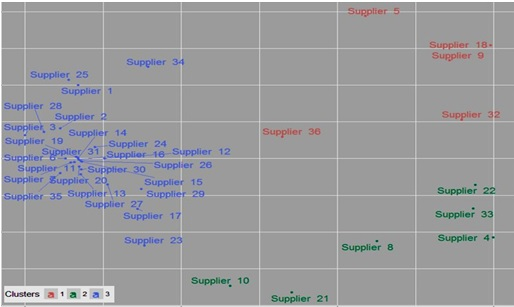
\includegraphics[width=1.0\textwidth]{Cluster.jpg}
	%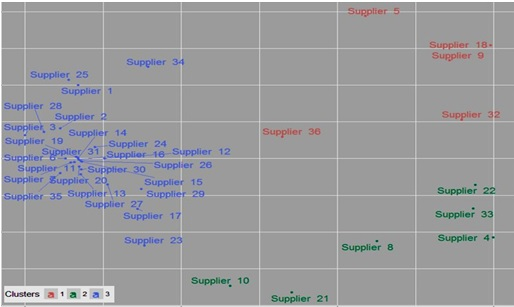
\includegraphics{Cluster.jpg}
    \caption{Clustering Suppliers by their Business Attributes }
    \label{fig:fig3}
\end{figure}

Figure \ref{fig:fig3} shows an example of the supplier clustering for suppliers listed in  Figure \ref{fig:fig1} which has three distinct clusters, color coded as blue, green and red. The shape of a cluster is due to business attributes of its member suppliers. Therefore, rationalizing suppliers within their own clusters will be easier than rationalizing suppliers between clusters since members of the same cluster can absorb others' volume with the least amount of impact to Verizon's sourcing operations and help supplier consolidation. Identifying rationalization candidates still is not a trivial task at this stage as each one of these suppliers provides Verizon with multiple categories of products and services. That being said, more detailed analyses are needed for Verizon sourcing teams to identify the right rationalization candidates. For example, comparing suppliers with their peers based on their KPIs and PPUs of sourced categories and items. The outputs of this stage are clusters of suppliers which can be compared with each other or with other clusters. 

\subsection{Optimization Models}
DEA works well for evaluating suppliers across multiple categories with their peers. DEA establishes relationships between inputs and outputs of the suppliers and evaluates all of the other suppliers with the efficient frontier supplier, a supplier that provides the best PPU and KPI (or any other metrics) in that category compared to its peers. Higher inputs to a supplier calls for higher outputs and performance.

The inputs to suppliers can be annualized PO values sent to a supplier and outputs can be PPU of items purchased and procurement KPIs. Table \ref{tabel:tbl3} reviews some of the procurement KPIs which are considered by Verizon contract management teams when evaluating suppliers and used in the developed DEA model. The developed DEA model in this paper establishes inverse relationships its inputs and outputs as the higher the spend with a supplier is, the lower the KPIs and PPUs should be. DEA models can take different inputs and outputs. Readers can refer to \cite{r3}, to investigate the appropriate model orientations for their use case.

\begin{center}
\begin{table}
	\begin{tabular}{>{\centering\arraybackslash}m{5 cm} | >{\centering\arraybackslash}m{11 cm}}
	\multicolumn{2}{c}{}\\
	\hline
	KPI & Definition \\ 
	\hline
	\multirow{6}{*}{} 
	Delivery Lead Time Accuracy & Lead time variance of product or service deliveries to Verizon  specified location (non-carrier) \\
 	Fill Rate Accuracy & Percentage of POs not fulfilled by a supplier regardless of lead time \\
 	Number of Defects & Total number of SKUs with defects when inspected by Verizon engineers \\
 	Return Rate & Total number of SKUs returned due to technical mismatch with PO \\
 	Price Accuracy & Total financial value of invoice vs contract price variance \\ 
 	Quantity Accuracy & Variance between PO quantity and delivered quantity \\
	\hline
	\end{tabular}
	\caption{Important Supplier KPIs Used by Verizon's Strategic Sourcing Teams}
	\label{tabel:tbl3}
\end{table}
\end{center}

For this stage, the goal is to calculate an efficiency score, within each cluster, for each supplier and category combination, in turning financial resources and POs to the lowest levels of PPUs of items and KPIs for Verizon. The two-dimensional scoring matrix shown in Figure \ref{fig:fig4} is the resulting output of the DEA model for suppliers in the same cluster. Appendix B provides a detailed explanation of the mathematical optimization model, used to calculate the Figure \ref{fig:fig4} scoring matrix.

\begin{figure}
	%\centering
	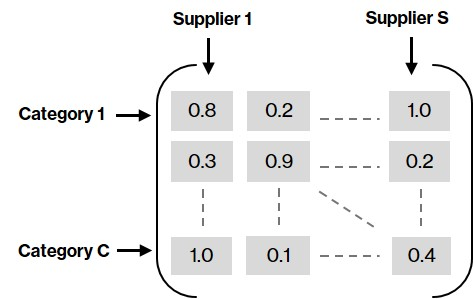
\includegraphics[width=0.5\textwidth]{ScoringMatrixBW.jpg}
    \caption{Example of Suppliers' Efficiency Score Matrix}
    \label{fig:fig4}
\end{figure}

Let $D^{g}$ be the mathematical model for a cluster of suppliers, $g$, where it compares the suppliers' inputs to their outputs subject to a group of business constraints. The mathematical problem, $D^{g}$, needs to be solved to optimality iteratively, i.e. once per Supplier, $s$, and Category $c$. The resulting scoring matrix of Figure \ref{fig:fig4} can be used to identify suppliers with low efficiency for turning inputs to outputs within any categories. Once the dimensions of this matrix increase (i.e. more suppliers and categories are added), category sourcing managers will have difficulties following the insights and directions of this matrix. Thus, even with the information provided by the efficiency matrix, identifying rationalization candidates is still difficult as the results of this matrix could be could interpreted differently by different category managers. In reality, no category manager wants to rationalize their managed suppliers or sourcing categories since this could jeopardize their careers. Therefore, discussions about rationalizing suppliers between sourcing teams and business units are often unproductive and biased. 

To avoid running into this situation and to facilitate a data-driven conversation between sourcing teams and business units when identifying rationalize candidates, an objective unbiased approach is required. The output of this stage is the suppliers' efficiency score matrix. The next section will cover details of the unbiased approach used within VSRT's optimization engines to solve this problem. 

\subsection{Biases in Supplier Ranking}
The subjectivity of identifying and evaluating candidate suppliers for rationalizing is often addressed with a Balanced Scorecard \citep{r7}, where a list of suppliers are scored by subject matter experts across various criteria and metrics. The results of these individual evaluations will then get aggregated and reported to decision makers as a ranking score. Such an approach is highly biased and subject to the tenure and expertise of evaluating individuals. Also this approach does not differentiate between suppliers which provide high risk and expensive categories, which are business sensitive, compared to other categories. For instance, suppliers with Active Cellsite Equipment (ACE) category in their portfolio have more exposure to supply disruption than the ones with Minor Material (i.e. nuts and bolts) categories. Thus, Verizon's risk tolerance for the ACE category suppliers is a lot smaller than the Minor Materials category suppliers. A traditional scorecard might allocate the same importance weight to suppliers with ACE category as to Minor Material's suppliers and recommend unrealistic supplier ranking. This issue calls for a reliable, holistic and objective evaluation approach for final supplier rationalization recommendations.

In order to provide an objective approach when identifying candidates for supplier rationalization, another set of algorithms have been used, taking into account Verizon sourcing managers' business acumen as well as transaction level supplier spend data. A novel method based on the Technique for Order Preference by Similarity to Ideal Solution (TOPSIS) \citep{r4} is used to solve the problem of ranking rationalization candidates based on their score of efficiency in each category as well as a set of additional business constrains, i.e. benefit and cost criteria. 

The idea behind TOPSIS is as follow: The best alternative supplier to a rationalization candidate would be a supplier which maximizes the benefit criteria and minimizes the cost criteria. The goal of this stage is to rank suppliers according to their 1) score of efficiency, 2) benefits and 3) cost criteria. Suppliers with lower ranks are candidates to rationalize. However, as it was mentioned earlier, Verizon strategic sourcing teams might value each category differently. Suppliers with higher spends in specific categories might have a higher risk to rationalize regardless of their performance efficiency. Therefore, different weights could be assigned in evaluating each category.

In order to use the TOPSIS algorithm, a supplier Decision Matrix (DM) needs to be created. Appendix C provides a detailed explanation of the DM, $D$, composite and its dimensions. In addition, the suppliers' efficiency score matrix could be used to fill in the entries of the decision matrix (i.e. $D$) and subject matter expertise of the Verizon sourcing teams could be leveraged to populate the weight matrix (i.e. $W$). Similar to the Balanced Scorecard, this approach will be highly subjective as every sourcing team values their categories and suppliers more than other teams' categories and suppliers. To avoid this highly biased approach, rather than using Verizon's subject matter inputs to populate the weight matrix, transaction level spend data and Shannon Entropy were used to normalize the weighting matrix, $W$. Following the steps of the TOPSIS algorithm and using the weight matrix, the supplier efficiency score matrix and the business criteria, the overall efficiency score of the suppliers across all the sourcing categories can be calculated. Readers can refer to \citep{r4} for the details of the TOPSIS algorithm implementation steps. The output of this stage is final supplier ranking for rationalization. The next section, provides discussions on the results of implementing this end-to-end solution. 

\section{Solution Results}
The VSRT is implemented on a Hadoop Supplier Cluster and a Hive environment \citep{r15} where most of the Verizon spend transaction data is stored. All Machine Learning Models including NLP, RNNs and Unsupervised Learning models were implemented in Python 3.6 \citep{r16}. The DEA model is solved using the IBM CPLEX 12.6 optimization engine \citep{r13}. Advanced interactive visualizations and executive dashboards were built using Qlik \citep{r14}. Transaction level data from FY2016 through the end of FY2018 were used to build input data models.

To demonstrate results of this solution, suppliers in Cluster number 2 of Figure \ref{fig:fig3} are selected. Table \ref{tabel:tbl4} includes the result of applying the presented methodology to all of the suppliers within Cluster 2. Suppliers 6, 17 and 22 are good rationalization candidates since their overall efficiency score across all the categories they provide is lowest among their peers.  

Verizon sourcing teams could then take the Table \ref{tabel:tbl4} results and start negotiating with the alternative suppliers, conducting RFPs and sourcing operations to move the business volume while the business units' planning teams update ERP systems and the budgeting. Now that the rationalization candidates are finalized, the next step is selecting alternative suppliers which can absorb the rationalized suppliers' business volume while providing better pricing (i.e. PPU) and service quality (i.e. KPIs).

\begin{center}
	\begin{table}
		\begin{tabular}{c|c|c|c}
			\multicolumn{4}{ c } {}\\
			\hline
			Supplier & Ranking & Overall Efficiency Score & Annualized Spend (\$M) \\ 
			\hline
			 Supplier 20 & 1 & 0.63 & 2.70 \\
			 Supplier 13 & 2 & 0.61 & 2.60 \\ 
			 Supplier 36 & 3 & 0.59 & 0.40 \\ 
			 Supplier 35 & 4 & 0.55 & 2.40 \\ 
			 Supplier 32 & 5 & 0.51 & 0.10 \\ 
			 Supplier 29 & 6 & 0.47 & 1.00 \\ 
			 Supplier 6 & 7 & 0.44 & 0.50 \\ 
			 Supplier 17 & 8 & 0.36 & 0.36 \\ 
			 Supplier 22 & 9 & 0.15 & 0.15 \\			
			\hline
		\end{tabular}
		\caption{Long Tail Suppliers Ranking for Rationalization}
		\label{tabel:tbl4}
	\end{table}
\end{center}

Knowing the historical order volume, $Q$, and new Price Per Unit, $nppu$, for an SKU, $u$,  new supplier spend (i.e. $nppu_{u} \times Q_{u}$) can be calculated post rationalization. The Alternative Suppliers' Matrix and this new supplier spend can be used to identify alternative suppliers for the rationalized suppliers. Figure \ref{fig:fig5} shows the SAM for the suppliers in Table \ref{tabel:tbl4}, where positive financial impacts of moving volume from a rationalized candidate supplier to an alternative supplier are illustrated in green and the negative overall impact is shown in red. These financial impacts are calculated across all of the categories and items provided by the suppliers. 

\begin{figure}
	%\centering
	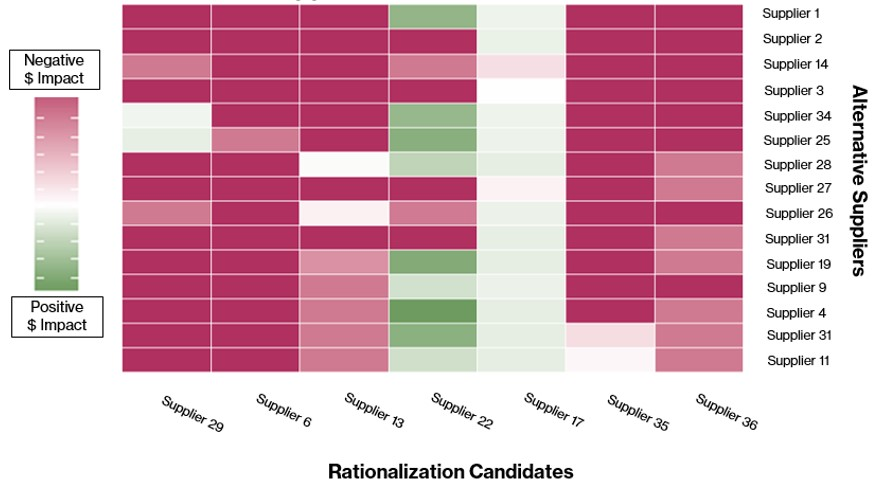
\includegraphics[width = 0.9\textwidth]{SupplierAlternativeMatrixBW.jpg}
    \caption{Alternative Suppliers' Matrix}
    \label{fig:fig5}
\end{figure}


\begin{center}
	\begin{table}
		\begin{tabular}{>{\centering\arraybackslash}m{4 cm}|
		>{\centering\arraybackslash}m{4.3 cm}|
		>{\centering\arraybackslash}m{4.3 cm}}
		\multicolumn{3}{c}{} \\
		\hline
		Manufacturer Part Number & PPUV Before Rationalization & PPUV After Rationalization \\ 
		\hline
		Part 1 & 32\% & 0\% \\
		Part 2 & 32\% & 31\% \\
		Part 3 & 31\% & 0\% \\
		Part 4 & 24\% & 0\% \\
		Part 5 & 23\% & 0\% \\
		Part 6 & 14\% & 0\% \\
		Part 7 & 14\% & 0\% \\
		Part 8 & 14\% & 11\% \\
		Part 9 & 14\% & 0\% \\
		Part 10 & 13\% & 3\% \\
		Part 11 & 10\% & 0\% \\
		Part 12 & 9\% & 0\% \\
		Part 13 & 8\% & 6\% \\
		Part 14 & 8\%	& 0\% \\
		Part 15 & 8\% & 15\% \\
		Part 16 & 7\% & 19\% \\
		Part 17 & 6\% & 0\% \\
		Part 18 & 5\% & 0\% \\
		Part 19 & 5\% &	0\% \\
		Part 20 & 3\% & 0\% \\
		\hline
		\textbf{Average} & \textbf{23\%} & \textbf{4.25\%} \\
		\hline
		\end{tabular}
		\caption{SKU Price Per Unit Variance Before and After Supplier Rationalization}
		\label{tabel:tbl5}
	\end{table}
\end{center}

The alternative suppliers' matrix is a powerful tool to provide insights on selecting alternative suppliers for the sourcing teams, hence it does not provide detailed information at the SKU level. Table \ref{tabel:tbl5} illustrates the impact of supplier rationalization at the SKU level to some of the sourced SKUs. The Price Per Unit Variance (PPUV) of most of these items reduced on average from 23\% to of 4.25\% post supplier rationalization, except for Part 15 and Part 16, where Verizon is getting a higher PPU due to volume consolidation and shift to alternative suppliers and missing the existing contractual price brackets with its current rationalized supplier. However, this variance was affordable as the overall portfolio of sourced SKUs was net positive after rationalization. The price variance is calculated comparing to the baseline unit price of the items. 

\section{Conclusion}
The implementation of this end-to-end solution was successful and eliminated tens of millions of dollars from Verizon bottom line expenses, while improving labor productivity and contract execution cycle times. This solution added value to the Verizon's Global Supply Chain organization from the start, providing clear directions, gaining trust among business partners and achieving strong executive support. While analytics was key for the success of this project, flawless execution by Verizon category sourcing managers and the trusted partnership built with suppliers also significantly influenced the business results.

The design of this solution was creative where different types of analytics were utilized in a unique sequence: 1) Natural Language Processing and Artificial Neural Networks were used to structure and transform Verizon's large scale unstructured spend data into high quality inputs for Machine Learning algorithms, 2) a blend of internal and external data sources were used to enrich the supplier segmentation and clustering, 3) Operations Research techniques were used in unique and innovative ways to generate insights and drive meaningful conversations when comparing suppliers at the category level, 4) Multi-Criteria Decision Making (MCDM) methodologies such as TOPSIS and Shannon Entropy were used to tackle bias with objective data-driven approaches, taking emotions out of supplier conversations and executive decisions, 5) advanced visualization was used to communicate the complex algorithms and their results to our business partners so that they were able to understand and accept our recommendations.

This solution provided a fast and efficient toolset to perform supplier rationalization for Verizon strategic sourcing teams and tremendously helped supplier negotiations, the RFP process, Linear Price Performance and Similar Part Analysis. Supplier negotiations and execution of this solution's recommendations are strategic and long term. Thus, more financial benefits are expected to be realized over time as the solution is rolled out when a majority of large contracts is renegotiated and volumes are further consolidated.

\section*{Acknowledgment}
The Verizon team and this paper were the third place winner of the 2019 INFORMS Innovative Applications in Analytics Award (IAAA) held in Austin TX. The authors would like to thank the 2019 IAAA committee members and judging panel: Juan Jaramillo, Aly Megahed, Erick Wikum, Micheal Gorman and Pallav Chhaochhria for their dedication, event coordination and the opportunity provided to Verizon for presenting this work. Special thanks to the Verizon coach, Lana Yeganova, for her tireless efforts on coaching us for the 2019 competition. Also to the two anonymous reviewers for their comments on earlier versions of this manuscript. Their comments improved this manuscript significantly. And to all VTeamers across the globe for providing a world-class customer service to Verizon customers. All errors are the authors' own. Information contained herein is provided AS IS and subject to change without notice.  All trademarks used herein are property of their respective owners.

\newpage
\begin{APPENDICES}
\section{Appendix A. Problem Formulation}
In order to formulate this business problem in simple mathematical terms, the following mathematical sets and indices need to be defined:
\begin{itemize}
\item[] $s \in {S}$: Suppliers (VARs, OEMs, etc.) 
\item[] $c \in {C}$: Product or Service Category	
\item[] $u \in {U}$: SKU or Item
\item[] $k \in {K}$: KPI
\item[] $ppu_{u}$: Price Per Unit of item $u$
\item[] $PPU_{c}$: Price Per Unit of a Category $c$
\item[] $Q_{u}$: Quantity of item $u$ sourced from a supplier
\end{itemize}

\vspace{0.25 in}

With the help of the above notations and indices, the following definition can define this problem in mathematical notations:

\begin{definition}
Define $s\textprime$ as $s\textprime = \{ s\textprime \subseteq S \hspace{2 mm} | \hspace{1 mm} s\textprime_{k} = \underset{s}{\mathrm{max}} \hspace{2 mm} s_{k} \hspace{2 mm}, \hspace{2 mm} s\textprime_{PPU_{c}} = \underset{s}{\mathrm{min}} \hspace{1 mm} s_{PPU_{c}} \hspace{2 mm} \forall c, k \} $ where $PPU_{c} = \frac{\sum_{u} Q_{u}{ppu_{u}}}{\sum_{u} Q_{u}} \hspace{3 mm} \forall c$, $ |s^{\prime}| \leq |S|$ and $s\textprime \neq \O $.
\end{definition}


\section{Appendix B. Optimization Model Formulation}
A Linear Programming (LP) optimization model has been formulated to score suppliers in each category within each cluster. Let problem $D^{g}$ be the DEA optimization model used for evaluating suppliers within each cluster $g$. Problem $D^{g}$ is the dual of the primal DEA model. This dual model is easier for the business users to follow. Readers can refer to available literature \citep{r12} to investigate the primal formulation. The following notations are utilized to describe the optimization model $D^{g}$ formulation:\\

\noindent \textbf{Indices and Parameters:}
\begin{itemize}
\item[] $g$: A group or a cluster of suppliers
\item[] $\epsilon$: Very small positive number
\item[] $i$: Vector of inputs to suppliers (Number of POs, PO Values, Supplier Spend and etc.)
\item[] $o$: Vector of outputs from suppliers (Fulfilled POs, Provided PPU and etc.)
\item[] $s^0$: Supplier under consideration (Current DMU)
\item[] $x_{is}^c$: Amount of input (POs or PO Values) used by supplier $s$ in category $c$
\item[] $y_{os}^c$: Amount of output (KPIs and PPU) generated by supplier $s$ in category $c$
\end{itemize}

\vspace{.5 cm}

\noindent \textbf{Decision Variables:}
\begin{itemize}
\item[] $\theta_{s}^c$ : Score of efficiency of supplier $s$ in category $c$ 
\item[] $\lambda_{s}^c$ : Weight coefficient of supplier $s$ in category $c$ 
\item[] $Slack_{i}^{c}$ : Auxiliary variable for input $i$ shortage in category $c$
\item[] $Surplus_{o}^{c}$ : Auxiliary variable for output $o$ surplus in category $c$ 
\end{itemize} 

\begin{align} 
D^{g}: \quad \text{MIN } & \theta_{s^0}^{c} - \epsilon \hspace{1 mm} \Bigg[\sum_{i \hspace{1 mm}\in \hspace{1 mm} inputs} Slack_{i}^{c} \hspace{2 mm} + \sum_{o \hspace{1 mm} \in \hspace{1 mm} outputs} Surplus_{o}^{c} \hspace{1 mm} \Bigg ] \label{e1} \\ 
\text{s.t. } & \sum_{s \in S} \lambda_{s}^c \hspace{1 mm} x_{is}^c \hspace{1 mm} + \hspace{1 mm}Slack_{i}^{c} \hspace{1 mm} = \hspace{1 mm} \theta_{s^0}^c \hspace{1 mm} x_{i{s}^o}^c \hspace{.3in} \forall c, i, s^0 \in S\label{e2}\\
& \sum_{s \in S} \lambda_{s}^c \hspace{1 mm} y_{os}^c \hspace{1 mm} - \hspace{1 mm}Surplus_{o}^{c} \hspace{1 mm} \geq \hspace{1 mm} \theta_{s^0}^c \hspace{1 mm} y_{o{s}^o}^c \hspace{.3in} \forall c, o, s^0 \in S \label{e3}\\
& \lambda_{s}^{c}, \hspace{1 mm} Surplus_{o}^{c}, \hspace{1 mm} Slack_{i}^{c} \hspace{1 mm}  \geq 0 \hspace{.3in} \forall s, c, o, i , s \in S\label{e4}\\
& 1 \geq \theta_{s^0}^{c} \geq 0 \hspace{.3in} \forall s^0, c, s^0 \in S \label{e5}
\end{align}

The problem $D^{g}$ needs to be solved for each cluster of suppliers separately as it is problematic to compare suppliers which do not provide Verizon with similar categories. Objective function \eqref{e1} minimizes the sum of Slack inputs (i.e. PO values) to suppliers and Surplus outputs (i.e. PPUs and KPIs) from suppliers in across each sourcing category. In the best case scenario, current DMU $s^0$ has no excess in using inputs but has as much excess outputs as possible.  

In order to constraint supplier excess and shortage of inputs and outputs, a set of constraints needs to be included to the model $D^{g}$. When comparing supplier $s^0$ with its peer suppliers $s$ within a category $c$, constraints \eqref{e2} ensure that there will be no surplus of inputs to the supplier $s^0$  while constraints \eqref{e3} ensure that there is no shortage of outputs from the supplier in comparison to its peers. Constraints \eqref{e4} and \eqref{e5} are feasibility constraints indicating that $\lambda_{s}^{c}, \hspace{1 mm} Surplus_{o}^{c}, \hspace{1 mm} Slack_{i}^{c}$ are continuous and non-negative, and $\theta_{s^0}^{c}$ is between 0 and 1.\\

\section{Appendix C. TOPSIS Decision Matrix}
Let $A$ be a set of alternative suppliers to the rationalization candidates which can absorb the volume of rationalized suppliers. This is the supplier set toward the head spend of Figure \ref{fig:fig1}. Let $L$ also be a set of criteria where the sourcing teams are interested in (e.g. lead time for delivering products in a category must be less than 45 days, etc.). A decision matrix, $D$, can be built similar to Figure \ref{fig:fig4} where rows are alternative suppliers and columns are criteria. Let matrix $W$ be the weighting matrix for each criterion where rows and columns are alternative suppliers and sourcing categories and $\sum_{c \in C} \sum_{s \in S}{w^{cs}}= 1 \hspace{1 mm} \forall \hspace{2 mm} l \in L$. The supplier efficiency score matrix, $e$, which has the same dimensions as the weighting matrix $W$, can be blended to create the decision matrix $D$. Figure \ref{fig:figDM} illustrates this matrix where each row is an Alternative Supplier, $a$, and the each column is a criterion, $l$.  

\begin{figure}
	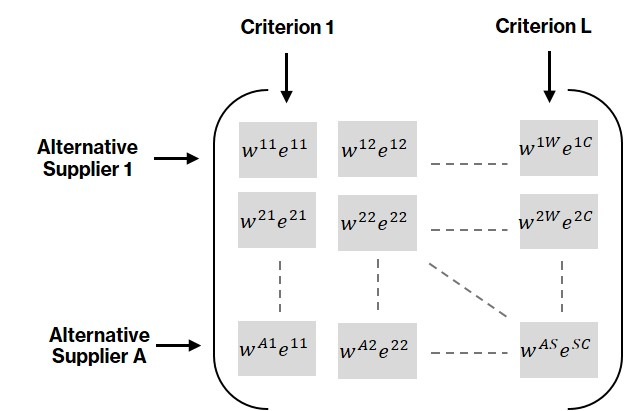
\includegraphics[width=0.5\textwidth]{DecisionMatrix.jpg}
    \caption{The Decision Matrix Composite Structure}
    \label{fig:figDM}
\end{figure}

\end{APPENDICES}

\newpage

\bibliographystyle{informs2014}
%\bibliography{TailSpend}
\newcommand{\comment}[1]{}

\begin{thebibliography}{}
\bibitem[Hive, 2018]{r15}{Apache Hive (2018) Hive Developer Documentation, http://hive.apache.org/.}
\bibitem[Bayrak et al., 2007]{r30}{Bayrak MY, Celebi N, Taskin H (2007) A fuzzy approach method for supplier selection. \textit{Production Planning \& Control}. 18(1):54-63.} 
\bibitem[Bilsel et al., 2006]{r36}{Bilsel RU, Buyukozkan G, Ruan D (2006) A Fuzzy Preference-Ranking Model for a Quality Evaluation of Hospital Web Sites. \textit{International Journal of Intelligent Systems}. 21(11):1181-1197.}
\bibitem[Charnes et al., 1978]{r12}{Charnes A, Cooper WW, Rhodes E (1978) Measuring the Efficiency of Decision Making Units. \textit{European Journal of Operational Research}. 2(6):429-444.}
\bibitem[Cook et al., 2014]{r3}{Cook WD, Tone K, Zhu J (2014) Data Envelopment Analysis: Prior to Choosing a Model. \textit{OMEGA}. 44:1-4.}
\bibitem[Doyle et al., 1994]{r21}{Doyle J, Green R (1994) Efficiency and cross-efficiency in DEA: Derivations, meanings and uses. \textit{Journal of Operational Research Society}. 45(5):567-578.}
\bibitem[Ellram et al., 2015]{r23}{Ellram L, Tate W (2015) Redefining Supply Management's Contribution in Services Sourcing. \textit{Journal of Purchasing \& Supply Management}, 21:64-78.}
\bibitem[Feeny et al., 2005]{r26}{Feeny D, Lacity M, Willcocks LP (2005) Taking the Measure of Outsourcing Providers. \textit{MIT Sloan Management Review}. 46(3):41-48.}
\bibitem[Furnkranz, 1999]{r9}{Furnkranz J (1999) Pruning Algorithms for Rule Learning. \textit{Machine Learning}. 27:139-172.}
\bibitem[Geiger, 2012]{r11}{Geiger BC, Kubin G (2012) Relative Information Loss in
the PCA. \textit{Proceedings of IEEE Information Theory Workshop (ITW), Lausanne, Switzerland}. 562-566.}
\bibitem[Hwang et al., 1993]{r4}{Hwang CL, Lai YJ, Liu TY (1993) A New Approach for Multiple Objective Decision Making. \textit{Computers and Operational Research}. 20:889-899.}
\bibitem[IBM, 2017]{r13}{IBM (2017) IBM ILOG CPLEX 12.7 User’s Manual (IBM ILOG CPLEX Division, Incline Village, NV).}
\bibitem[Kaplan, 1992]{r7}{Kaplan RS, Norton DP (1992) The Balanced Scorecard - Measures That Drive Performance. \textit{Harvard Business Review}. 71-79.}
\bibitem[Kleinsorge, 1992]{r19}{Kleinsorge IK, Schary PB, Tanner RD (1992) Data Envelopment Analysis for Monitoring Customer Supplier Relationships. \textit{Journal of Accounting and Public Policy}. 11:357-372.}
\bibitem[Loader, 2015]{r24}{Loader, K (2015) SME Suppliers and the Challenge of Public Procurement: Evidence Revealed by a UK Government Online Feedback Facility. \textit{Journal of Purchasing \& Supply Management}. 21:103-112.}
\bibitem[Manning et al., 1999]{r10}{Manning CD,  Schütze H (1999) Foundations of statistical natural language processing, \textit{MIT press}.}
\bibitem[Narasimhan et al., 2001]{r20}{Narasimhan R, Talluri S, Mendez D (2001) Supplier Evaluation and Rationalization via Data Envelopment Analysis: An Empirical Examination. \textit{Journal of Supply Chain Management}. 37(3):28-37.}
\bibitem[Narasimhan et al., 2006]{r31}{Narasimhan R, Talluri S, Mahapatra SK (2006) Multiproduct, Multicriteria Model for Supplier Selection with Product Life-cycle Considerations. \textit{Decision Sciences}. 37(4):577-603.}
\bibitem[Python, 2018]{r16}{Python (2018) The Python Language Reference, https://docs.python.org/3.6/reference/.}
\bibitem[Qlik Sense, 2017]{r14}{Qlik Sense (2018) Qlik Sense Desktop, http://help.qlik.com/en-US/sense/.}
\bibitem[Rao et al., 2010]{r29}{Rao C, Xiao X, Goh M, Zheng J, Wen J (2017) Compound Mechanism Design of Supplier Selection Based on Multi-attribute Auction and Risk Management of Supply Chain. \textit{Computers \& Industrial Engineering}. 105:63-75.}
\bibitem[Rencher, 2002a]{r1}{Rencher AC (2002a) Methods of Multivariate Analysis (pp.380-387), \textit{Wiley Series in Probability and Statistics}.}
\bibitem[Rencher, 2002b]{r2}{Rencher AC (2002b) Methods of Multivariate Analysis (pp.482-488), \textit{Wiley Series in Probability and Statistics}.}
\bibitem[Rendle, 2010]{r8}{Rendle S (2010) Factorization Machines. \textit{In Proceedings of the 10th IEEE International Conference on Data Mining}. IEEE Computer Society. 995-1000.}
\bibitem[Sarkara et al., 2006]{r22}{Sarkara A, Mohapatrab PKJ (2006) Evaluation of Supplier Capability and Performance: A Method for Supply Base Reduction. \textit{Journal of Purchasing \& Supply Management}. 12:148-163.}
\bibitem[Schmidhuber, 1993]{r5}{Schmidhuber J (2015) Deep Learning in Neural Networks: An Overview. \textit{Neural Networks}. 61:85-117.}
\bibitem[Shannon, 1948]{r6}{Shannon CE (1948), A Mathematical Theory of Communication. \textit{Bell System Technical Journal}. 27(3):379-423.}
\bibitem[Talluri et al., 2003]{r17a}{Talluri S, Narasimhan R (2003) Vendor Evaluation with Performance Variability: A Max–Min Approach. \textit{European Journal of Operational Research}. 146(3):543-552.}
\bibitem[Talluri et al., 2004]{r17}{Talluri S, Narasimhan R (2004) A Methodology for Strategic Sourcing. \textit{European Journal of Operational Research}. 154:236-250.}
\bibitem[Talluri et al., 2010]{r32}{Talluri S, Lee JY (2010) Optimal supply contract
selection. \textit{International Journal of Production Research}. 48(24):7303-7320.}
\bibitem[Talluri et al., 2013]{r33}{Talluri S, DeCampos HA, Hult GTM (2013) Supplier Rationalization: A Sourcing Decision Model. \textit{Decision Sciences}. 44(1):57-86.}
\bibitem[Taha, 1975]{r34}{Taha H A (1975) Integer Programming: Theory, Applications, and Computations (pp. 1-30), \textit{Academic Press Inc.}.}
\bibitem[Yoon et al., 2018a]{r25}{Yoon J, Rosales C, Talluri S (2018) Inter-Firm Partnerships-Strategic Alliances in the Pharmaceutical Industry. \textit{International Journal of Production Research}. 56(1-2):862-881.}
\bibitem[Yoon et al., 2018b]{r27}{Yoon J, Talluri S, Yildiz H, Ho W (2018) Models for
supplier selection and risk mitigation: a holistic Approach. \textit{International Journal of Production Research}. 56(10):3636-366.}
\bibitem[Wu et al., 2010]{r28}{Wu DD, Olson D (2010) Enterprise Risk Management: A DEA VaR Approach in Vendor Selection. \textit{International Journal of Production Research}. 48(16):4919-4932.}
\end{thebibliography}





% Acknowledgments here
%\ACKNOWLEDGMENT{}
% Leave this (end of acknowledgment)


% Appendix here
% Options are (1) APPENDIX (with or without general title) or 
%             (2) APPENDICES (if it has more than one unrelated sections)
% Outcomment the appropriate case if necessary
%
% \begin{APPENDIX}{<Title of the Appendix>}
% \end{APPENDIX}
%
%   or 
%
% \begin{APPENDICES}
% \section{<Title of Section A>}
% \section{<Title of Section B>}
% etc
% \end{APPENDICES}


% References here (outcomment the appropriate case) 

% CASE 1: BiBTeX used to constantly update the references 
%   (while the paper is being written).
%\bibliographystyle{informs2014} % outcomment this and next line in Case 1
%\bibliography{<your bib file(s)>} % if more than one, comma separated

% CASE 2: BiBTeX used to generate mypaper.bbl (to be further fine tuned)
%\input{mypaper.bbl} % outcomment this line in Case 2

\end{document}


